This sections aims to describe the notion of topological invariant and its consequence on the band structure. 
\subsection{Topological equivalence of insulators \label{subsec:Top_Band}}
In a periodic lattice potential, electrons are described by bloch states $\ket{n, \mathbf{k}}$ where $n$ is a dicrete quantum number and $\mathbf{k}$ is the crystal momentum in the brillouin zone \cite{girvin_modern_2019}. Each of those states is associated to an energy $E_{n, \mathbf{k}}$.  As it varies with $\mathbf{k}$, the energy sweeps a continous range called a band labeled with the number $n$. Bands are often separated by energy gaps where there are no associated states. Trivial insulators have a gapped ground state meaning that low energy excitations are forbidden by the presence of the gap. On the contrary, topological insulators have metallic (gapless) edge states\cite{kane_topological_2013} and different from trivial insulators in a fundamental way.\\ 


The adiabatic theorem tells us that sufficiently slow modifications of the hamiltonian of a trivial insulator will change its band structure while leaving it in its ground state\cite{born_beweis_1928}. This \textit{deformation} is said to yield equivalent insulators if the gap doesn't close \cite{kane_topological_2013}. This equvalence is topological in the same way the continuous disformation from a torus to a coffee mug is. Just like the coffee mug cannot be continuously deformed into a sphere, a trivial insulator cannot be continuously \textit{deformed} into a topological insulator.\\

% For the coffee mug and the sphere, a number tells if there is topological equivalence or not.
A coffee mug and a sphere are considered topologicaly different because they do not have the same number of holes, meaning you can't smoothly deform one into the other. 
This number (of holes) is called the genus and it as analogues for topological insulators \cite{batra_physics_2020}. The central property of genus is that it only changes when the torus is broken into a sphere in a necessarly discontinuous way. %Therefore, the genus is a topological invariant for the sphere and torus.
For the QHE the relevant topological invariant %indicating the persistance of the edge states 
(under deformation of the Hamiltonian) is the Chern number. For the QSH effect, a $\mathbb{Z}_2$ invariant is involved \cite{kane_topological_2013}. In the following section, the link between time reversal symmetry and this last invariant is detailed.  Mixing symmetry, topological invariants and dimensionnality allows for a classification of topological insulators in a sort of \textit{periodic table} \cite{hasan_topological_2010}. 

\subsection{Time reversal symmetry}
In a quantum mechanical setting, an operator $U$ (unitary or anti-unitary) corresponds to a symmetry of a system when $U H U^{-1} = H$ where $H$ is the hamiltonian governing the motion of the system. For a time reversal symetric (TRS) system this means that evolution follows the same equations of motion as a movie of itself set on rewind \cite{shankar_topological_2018}. The operator sending a system to its time reverse is an anti-unitary operator noted $\Theta$ and TRS corresponds to $\Theta H \Theta^{-1} = H$. In the position representation of the spin, momentum and position observables of an electron, the intuitive effects of this time reversal operator are the following \cite{shankar_topological_2018} : 
\begin{align*}
    \Theta \mathbf{s} \Theta^{-1} &=-\mathbf{s}, \\
    \Theta \mathbf{r} \Theta^{-1} &=\mathbf{r}, \\
    \Theta (-i\hbar\nabla) \Theta^{-1} &=+i\hbar\nabla
\end{align*}
meaning it sets electrons spinning backwards with a reversed velocity. The operator satisfying all those porperties is $\Theta = i s_y K$ where $K$ represents complex conjugation and the $i s_y$ factor ensures spin is fully reversed \cite{bernevig_topological_2013}. The essential property of the time reversal operator for electrons is that is satsifies $\Theta^2 = -1$. Hence reversing time twice for spin $1/2$ particles isn't the identity \cite{hasan_topological_2010}! This leads to Kramer's theorem which is said to be the most important theorem for time reversal invariant two dimensionnal topological insultors \cite{bernevig_topological_2013}. It states the following:\\

\fbox{\begin{minipage}{22em}
    \textbf{Kramer's Theorem: }For a time reversal invariant system containing an odd number of spin $1/2$ particles, there are at least two degenerate energy states \cite{bernevig_topological_2013}.
\end{minipage}}\\[0.3cm]

\begin{figure*}[!h]
    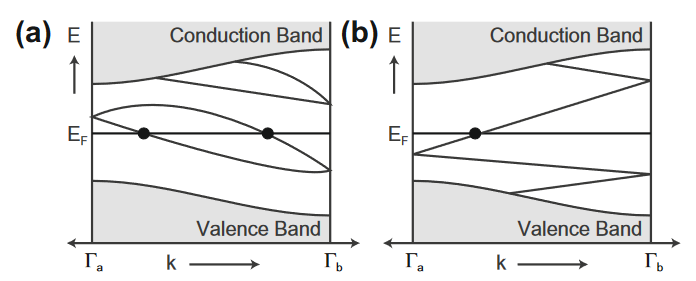
\includegraphics[scale = 0.8]{sections/visuel/kramer.png}
    \caption{Schematic representation of the two typical ways Kramer's theorem can be satisfied between TRIM points. (A) Shows a way to connect TRIM points without closing the gap. In this case there is an even amount of intersection points with the Fermi level. (B) Shows second way to connect TRIM points that closes the gap and has an odd number of intersections with the Fermi level \cite{kane_topological_2013}. To get a complete picture, on must keep in mind that the energies at $-\mathbf{k}$ are the same as the represented ones along the $k$ values of interest (they are Kramer degenerate).}
    \label{TRIM}
\end{figure*}

To use this theorem here, it must be applied to the periodic bloch states $\ket{n, \mathbf{k}}$ mentionned before. By bloch's theorem \cite{girvin_modern_2019}, these states can be written as the direct product $\ket{u_n(\mathbf{k})}\otimes \ket{\mathbf{k}}$ where $\ket{\mathbf{k}}$ takes care of the tranlsationnal symmetry of the crystal lattice and $\ket{u_n(\mathbf{k})}$ contains the details of the state over a unit cell. The basic idea of Kramers theoerem is that provided a state $\ket{u_n(\mathbf{k})}$, the action of the time reversal on it gives a state $\Theta\ket{u_n(\mathbf{k})}$ which has the same eigen energy as the first (if the hamiltonian is time reversal symmetric). Then, if there is no degeneracy the generated state must be related to the first one with a constant $c$ by $\Theta \ket{u_n(\mathbf{k})} = c \ket{u_n(\mathbf{k})}$ or else two physically different states would have the same energy\cite{kane_topological_2013}. Applying time reversal again yields
\begin{align*} 
    -\ket{u_n(\mathbf{k})} &= \Theta \{\Theta\ket{u_n(\mathbf{k})}\}\\ &= c^\star \Theta \ket{u_n(\mathbf{k})}\\ &= c c^\star \ket{u_n(\mathbf{k})}\\ &= |c|^2\ket{u_n(\mathbf{k})}
\end{align*}
where $c$ gets conjugated by $K$ and the porperty $\Theta^2 =-1$ was used. This series of equalities suggests that, if a state is non degenerate, $|c|^2 = -1$ which is impossible and leads to a contradtiction: the states must be twofold degenerate \cite{kane_topological_2013}. This can be made more precise by noting that the time reverse of $\ket{u_n(\mathbf{k})}$ is $\ket{u_{n'}(\mathbf{-k})}$ \cite{bernevig_topological_2013} (a state with reversed crystal momentum possibly living on a different band). Furthermore, the time reversed state also has reversed spin \cite{kruthoff_topology_2019}.\\

Special points called time reversal invariant momentas (TRIM) lead to a crucial effect of the theorem. They are points in the Brillouin zone that are sent to points with an equivalent cristal momentum by time reversal ($\mathbf{k} \equiv -\mathbf{k}$) \cite{kruthoff_topology_2019}. At TRIM points, the Kramer degeneracy can only be satisfied if the states come from $2$ defferent bands having different spins \cite{kruthoff_topology_2019}. This forces bands to touch at special points and then split as $\mathbf{k}$ varies trough the effect of spin orbit coupling \cite{kane_topological_2013}. In two dimensions, if there are edge states locked inside the gap of the bulk of an insulator, Kramer's theorem forces them to have one of two topologies represented on fig. \ref{TRIM} \cite{kane_topological_2013}. Consider the points having cristal momentum norm $k = 0$ ($\Gamma_a$) and the point $k = \pi/a$ ($\Gamma_b$) (with $a$ being the unit cell size in one direction): they are both TRIM points because $\mathbf{0} = - \mathbf{0}$ and $k = \pi/a$ is equivalent to $k = -\pi/a$. The edge states at the TRIM points must connect two bands by Kramer's theorem. They can either do it in a gapped way (see fig. \ref{TRIM} (A)) or in a metallic gapless way (see fig. \ref{TRIM} (B)).\\

While the band configuration in fig. \ref{TRIM} (A) can be gapped out by the addition of disorder (time reversal symmetric impurities \cite{asboth_short_2016}), configuration (B) always remain gapless and its metallic behavior is robust to deformations of the system (and of its Hamiltonian) \cite{cayssol_topological_2021}. This is where the word \textit{topological} insulator gets its meaning. To be more precise, disforming the band structure from $(A)$ to $(B)$ would requier closing the bulk gap or breaking TRS which would indicate a topological phase transition \cite{cayssol_topological_2021}. Just like it was mentionned in sec. \ref{subsec:Top_Band}, there is a number distinguishing between configuration (A) and (B) refered to as the $\mathbb{Z}_2$ topological invariant.\\

Since there are \textit{two} different ways to connect TRIM points, the invariant used to qualify the topology of a 2D TRS topological insulators is an integer $\nu$ taking values $0$ or $1$ \cite{bernevig_topological_2013}. If $\nu = 0$ then the band insulator is trivial and, if $\nu = 1$, it is topological \cite{cayssol_topological_2021}. To give precise meaning to this number, it suffice to use the notion of a \textit{Kramer pair}. Two states related to each other by the application of $\Theta$ are called a Kramer pair \cite{asboth_short_2016}. In fig. \ref{TRIM}, only one member of each Kramer pair is shown so it is important to Keep in mind that all points show effectively count for one pair. The $\nu$ invariant corresponds to the parity of the number of kramer pairs at a fixed energy \cite{asboth_short_2016}. If the number of pairs is even (A) then $\nu = 0$, the insulator is gapped and trivial. Otherwise the number of pairs is always odd (B) and the insulator is topological.


%Time reversal symmetry (TRS) plays an important role in QSH topological insulators: it protects the gapless edge states \cite{kane_topological_2013}. While the QH effect requiers a magnetic field to occur (breaking of TRS), the QSH effect doesn't and it preserves TRS\cite{cayssol_topological_2021}. 
